\documentclass[utf8]{beamer}

% Packages
\usepackage[T1]{fontenc}
\usepackage[francais]{babel}
\usepackage{array}
\usepackage{verbatim}
\usepackage{graphics} %inclusion de figures
\usepackage{graphicx} %inclusion de figures
\usepackage{pstricks,pst-node} %Graphiques
\usepackage{booktabs}
\usepackage{minted}
\usepackage{rotating}
\usepackage{wrapfig}
\usepackage{graphicx}
\usepackage[inline]{asymptote} 
\usepackage{amsmath}
\usepackage{amsfonts}
\usepackage{amssymb}
\usepackage{amsthm}
\newcommand{\eod}{\ensuremath{\hfill\dashv}}
\newcommand{\eop}{\ensuremath{\hfill\clubsuit}}
\newcommand{\fun}[1]{\ensuremath{\mbox{\it #1}}}
\newcommand{\expo}[2]{{#1}^{\mbox{\scriptsize \sl #2}}}
\newcommand{\var}{\ensuremath{\mathbf{var}}\xspace}
\newcommand{\exv}{\ensuremath{\mathbf{exv}}\xspace}
\newcommand{\dsv}{\ensuremath{\mathbf{dsv}}\xspace}
\newcommand{\term}{\ensuremath{\mathbf{term}}\xspace}
\newcommand{\pred}{\ensuremath{\mathbf{pred}}\xspace}
\newcommand{\fr}{\ensuremath{\mathbf{fr}}\xspace}
\newcommand{\cnst}{\ensuremath{\mathbf{cnst}}\xspace}
\newcommand{\Vars}{\ensuremath{\mathsf{Vars}}\xspace}
\newcommand{\Pvars}{\ensuremath{\mathsf{Pvars}}\xspace}
\newcommand{\Fvars}{\ensuremath{\mathsf{Fvars}}\xspace}
\newcommand{\Terms}{\ensuremath{\mathsf{Terms}}\xspace}
\newcommand{\Cons}{\ensuremath{\mathsf{Const}}\xspace}
\newcommand{\Preds}{\ensuremath{\mathsf{Preds}}\xspace}
\newcommand{\ic}{\ensuremath{\cdot\{}\xspace}
\newcommand{\ci}{\ensuremath{\}\cdot}\xspace}
\newcommand{\id}{\ensuremath{:\hspace{-1.56mm}\{}\xspace}
\newcommand{\di}{\ensuremath{\}\hspace{-1.56mm}:}\xspace}
\newcommand{\bet}{\ensuremath{\beta^{\diamond}}\xspace}
\newcommand{\sep}{\ensuremath{\mathbf{sep}}\xspace}
\newcommand{\vect}[1]{\mathbf{#1}}
\newcommand{\vars}[1]{\fun{vars}{(#1)}}
\newcommand{\terms}[1]{\fun{terms}{(#1)}}
\newcommand{\atoms}[1]{\fun{atoms}{(#1)}}
\newcommand{\type}[1]{\fun{type}{(#1)}}
\newcommand{\const}{a}
\newcommand{\atom}{\alpha}
\usepackage{tikz}
\usetikzlibrary{arrows,positioning,automata,shadows,fit,shapes,calc, shapes, backgrounds}
\usepackage[linesnumbered,ruled,french,onelanguage]{algorithm2e}
\usepackage{hyperref}
\usepackage{setspace}

\newcolumntype{C}[1]{>{\centering\arraybackslash}p{#1cm}}

\newcommand{\pt}[5]{\dotnode(#2,#3){#1} \uput[#4](#2,#3){#5}}
\newcommand{\ptt}[5]{\dotnode(#2,#3){#1} \uput[#4](#2,#3){{\tiny #5}}}

% Style
\usepackage{pgfpages}
\usetheme{Montpellier}
\usecolortheme{whale}
\setbeamertemplate{footline}[page number]

% Informations
\title{Gestion des redondances dans les bases de connaissances}
\author{
  Leonardo \bsc{Moros} \\
  Guillaume \bsc{Perution-Kihli} \\
  Romain \bsc{Ricalens} \\
  Julien \bsc{Rodriguez} \\
  Rami \bsc{Younes}}

% Tableaux
\definecolor{GT1}{gray}{0.99}
\definecolor{GT2}{gray}{0.95}
\newcommand{\mc}[3]{\multicolumn{#1}{#2}{#3}}
\newcommand{\mr}[2]{\begin{tabular}[x]{@{}c@{}}#1\\#2\end{tabular}}
\newcolumntype{R}[1]{>{\raggedleft\arraybackslash}m{#1}}
\newcolumntype{L}[1]{>{\raggedright\arraybackslash}m{#1}}
%\newcolumntype{C}[1]{>{\centering\arraybackslash}m{#1}}

% Divers
\newcommand{\true}{\textcolor{orange}{1}}
\newcommand{\false}{\textcolor{orange}{0}}
\addto\captionsfrench{\def\figurename{{\bsc{Figure}}}}
\addto\captionsfrench{\def\tablename{{\bsc{Tableau}}}}

\begin{document}
\maketitle

\frame{\frametitle{Table des matières}\tableofcontents}

\section{Introduction}
    \begin{frame}{Qu'est-ce qu'une base de connaissances ?}
    \begin{itemize}
        \item<1-> Une base de faits - par exemple : $\mathcal{F} = enseigne(Jacques, algorithmique) \land suitCours(Julie, algorithmique)$
        \item<2-> Une base de règle - par exemple : $\mathcal{R} = \{\forall X,Y. aPourProf(X,Y) \rightarrow estProfDe(Y,X),\linebreak \forall X,Y,Z.suitCours(X,Y) \land enseigne(Z,Y) \rightarrow aPourProf(X,Z) \}$
    \end{itemize}
\end{frame}

\begin{frame}{Quel est l'intérêt ?}
    \begin{block}{Inférer des nouveaux faits de manière automatique}
         \only<2->{$\mathcal{F} = enseigne(Jacques, algorithmique) \land \linebreak suitCours(Julie, algorithmique)$ \\
         $\mathcal{R} = \{\forall X,Y. aPourProf(X,Y) \rightarrow estProfDe(Y,X),\linebreak \forall X,Y,Z.suitCours(X,Y) \land enseigne(Z,Y) \rightarrow aPourProf(X,Z) \}$ \\ 
         \only<3->{On peut inférer :\\ \only<3>{$aPourProf(Julie,Jacques)$} \only<4->{
            $aPourProf(Julie,Jacques), \linebreak estProfDe(Jacques, Julie)$\\
         }
         }
         }
         
         \only<5->{C'est du chaînage avant (\textit{chase}).}
    \end{block}
\end{frame}

\begin{frame}{Bases logiques}
    \begin{itemize}
        \item Logique du premier ordre sans symbole fonctionnel 
        \item Objets (termes) : \textbf{variables} et \textbf{constantes} 
        \item relations entre les termes : \textbf{prédicats} 
        \item \textbf{atome} : $p(t_1,\ldots,t_n)$
        \item \textbf{conjonction d'atomes} représentée par un \textbf{ensemble d'atomes} ;
    \end{itemize}
    
    \begin{block}{Exemple}
        $\exists X, p(a,b) \land p(b,X)$ devient $\{p(a,b),p(b,X)\}$
    \end{block}
\end{frame}

\begin{frame}[fragile]{Graphe associé à un ensemble d'atomes}
% Dans cette présentation, 2 représentations d'un ensemble d'atomes sont utilisées : graphe biparti et graphe orienté (arité < 2).

\begin{block}{Graphe biparti associé à $\mathcal{F} = \{p(a,b,X), q(b,X), p(X,Y,a)\}$}
\begin{asy}
// préambule asymptote
usepackage("amsmath,amssymb");
usepackage("inputenc","utf8");
usepackage("icomma");
// code figure
unitsize(1cm,1cm);
object sommet0=draw(Label("q"),ellipse,(0,0),NoFill);
object sommet1=draw(Label("X"),box,(2,0),NoFill);
object sommet2=draw(Label("Y"),box,(6,0),NoFill);
object sommet3=draw(Label("b"),box,(0,-2),NoFill);
object sommet4=draw(Label("a"),box,(4,-2),NoFill);
object sommet5=draw(Label("p"),ellipse,(2,-2),NoFill);
object sommet6=draw(Label("p"),ellipse,(4,0),NoFill);
add(new void(picture pic, transform t) {
path arete01=point(sommet0,dir(degrees((2,0),true)),t){dir(degrees((2,0),true))}..point(sommet1,dir(180+degrees((2,0),true)),t);
draw(pic,arete01);
label(pic,scale(.7)*"2",relpoint(arete01,.5),Relative(dir(90+degrees((2,0),true))),Fill(1,white));
path arete03=point(sommet0,dir(degrees((0,-2),true)),t){dir(degrees((0,-2),true))}..point(sommet3,dir(180+degrees((0,-2),true)),t);
draw(pic,arete03);
label(pic,scale(.7)*"1",relpoint(arete03,.5),Relative(dir(90+degrees((0,-2),true))),Fill(1,white));
path arete15=point(sommet1,dir(degrees((0,-2),true)),t){dir(degrees((0,-2),true))}..point(sommet5,dir(180+degrees((0,-2),true)),t);
draw(pic,arete15);
label(pic,scale(.7)*"3",relpoint(arete15,.5),Relative(dir(90+degrees((0,-2),true))),Fill(1,white));
path arete16=point(sommet1,dir(degrees((2,0),true)),t){dir(degrees((2,0),true))}..point(sommet6,dir(180+degrees((2,0),true)),t);
draw(pic,arete16);
label(pic,scale(.7)*"1",relpoint(arete16,.5),Relative(dir(90+degrees((2,0),true))),Fill(1,white));
path arete26=point(sommet2,dir(degrees((-2,0),true)),t){dir(degrees((-2,0),true))}..point(sommet6,dir(180+degrees((-2,0),true)),t);
draw(pic,arete26);
label(pic,scale(.7)*"2",relpoint(arete26,.5),Relative(dir(90+degrees((-2,0),true))),Fill(1,white));
path arete35=point(sommet3,dir(degrees((2,0),true)),t){dir(degrees((2,0),true))}..point(sommet5,dir(180+degrees((2,0),true)),t);
draw(pic,arete35);
label(pic,scale(.7)*"2",relpoint(arete35,.5),Relative(dir(90+degrees((2,0),true))),Fill(1,white));
path arete45=point(sommet4,dir(degrees((-2,0),true)),t){dir(degrees((-2,0),true))}..point(sommet5,dir(180+degrees((-2,0),true)),t);
draw(pic,arete45);
label(pic,scale(.7)*"1",relpoint(arete45,.5),Relative(dir(90+degrees((-2,0),true))),Fill(1,white));
path arete46=point(sommet4,dir(degrees((0,2),true)),t){dir(degrees((0,2),true))}..point(sommet6,dir(180+degrees((0,2),true)),t);
draw(pic,arete46);
label(pic,scale(.7)*"3",relpoint(arete46,.5),Relative(dir(90+degrees((0,2),true))),Fill(1,white));
});
shipout(bbox(0.1cm,0.1cm,white));
\end{asy}
\end{block}

\begin{block}{Graphe orienté associé à $\mathcal{F} = \{p(a,X), q(X,a), p(X,Y)\}$}
\begin{asy}
// préambule asymptote
usepackage("amsmath,amssymb");
usepackage("inputenc","utf8");
usepackage("icomma");
// code figure
unitsize(1cm,1cm);
object sommet0=draw(Label("a"),ellipse,(0,0),NoFill);
object sommet1=draw(Label("X"),ellipse,(2,0),NoFill);
object sommet2=draw(Label("Y"),ellipse,(4,0),NoFill);
add(new void(picture pic, transform t) {
path arete01=point(sommet0,dir(degrees((2,0),true)),t){dir(25+degrees((2,0),true))}..point(sommet1,dir(180+degrees((2,0),true)),t);
draw(pic,arete01,Arrow);
label(pic,scale(.7)*"p",relpoint(arete01,.5),Relative(dir(90+degrees((2,0),true))),Fill(1,white));
path arete10=point(sommet1,dir(degrees((-2,0),true)),t){dir(25+degrees((-2,0),true))}..point(sommet0,dir(180+degrees((-2,0),true)),t);
draw(pic,arete10,Arrow);
label(pic,scale(.7)*"q",relpoint(arete10,.5),Relative(dir(90+degrees((-2,0),true))),Fill(1,white));
path arete12=point(sommet1,dir(degrees((2,0),true)),t){dir(degrees((2,0),true))}..point(sommet2,dir(180+degrees((2,0),true)),t);
draw(pic,arete12,Arrow);
label(pic,scale(.7)*"p",relpoint(arete12,.5),Relative(dir(90+degrees((2,0),true))),Fill(1,white));
});
shipout(bbox(0.1cm,0.1cm,white));
\end{asy}
\end{block}


\end{frame}


\begin{frame}{Redondances}
    \begin{block}{Redondance}
    Un ensemble d'atomes S est redondant s'il existe un homomorphisme de S dans l'un de ses sous-ensembles stricts.
    \end{block}
    \begin{block}{Core}
    Un \textit{core} est un ensemble d'atomes non redondant.\\
    $Core(S)$ : sous-ensemble minimal de S équivalent à S.
    \end{block}
    \begin{block}{Exemple}
        $A = \{p(a,b),p(a,Y)\}$ contient une redondance. \\ \begin{tikzpicture}[->,>=stealth,shorten >=1pt,auto,node distance=2.5cm,
                thick,main node/.style={circle,draw,font=\Large\bfseries,scale=0.6}]
            \node[main node] (3) {$Y$};
            \node[main node] (1) [right of=3] {$a$};
            \node[main node] (2) [right of=1] {$b$};
            \path
                (1) edge node {$p$} (2)
                (1) edge node {$p$} (3);
        \end{tikzpicture}\\ 
        $Core(A) = \{p(a,b)\}$ \\
        \begin{tikzpicture}[->,>=stealth,shorten >=1pt,auto,node distance=2.5cm,
                thick,main node/.style={circle,draw,font=\Large\bfseries,scale=0.6}]
            \node[main node] (1) {$a$};
            \node[main node] (2) [right of=1] {$b$};
            \path
                (1) edge node {$p$} (2);
        \end{tikzpicture}\\
        
    \end{block}
\end{frame}

\begin{frame}{Homomorphisme}
    \begin{block}{Homomorphisme d'un ensemble d'atomes dans un autre} Soit $S$ et $S'$, deux ensembles d'atomes. Un homomorphisme est une substitution $h$ des variables de $S$ par des termes de $S'$ telle que $h(S) \subseteq S'$.
    %Si on voit les ensembles d'atomes comme une conjonction d'atomes fermée existentiellement, alors $S$ s'envoie par homomorphisme dans $S'$ si et seulement si $S$ est conséquence logique de $S'$. Ceci explique pourquoi l'homomorphisme est la notion fondamentale pour le cadre que nous étudions. En particulier deux ensembles d'atomes sont équivalents si chacun s'envoie dans l'autre par homomorphisme. Ici, on le note $S \rightarrow S'$.
    \end{block}
    \begin{block}{Propriété}
        $\exists h, h(S) \subseteq S' \Leftrightarrow S' \vDash S$
    \end{block}
    \begin{block}{Exemple}
        $A = \{p(Z,b),p(b,Y)\}$\\
        $B = \{p(a,b),p(b,X)\}$ \\
        Il existe un homomorphimse $h$ tel que $h(A) \subseteq B$ : $h = \{(Z \mapsto a), (Y \mapsto X)\}$.
    \end{block}
\end{frame}

% \begin{frame}{Base de connaissances}
%     \begin{block}{Base de connaissances}
%         Elle est composée d'une base de faits, qui est un ensemble d'atomes, et d'un ensemble de règles        Elle est composée d'une base de faits $\mathcal{F}$, qui est un ensemble d'atomes, et d'un ensemble de règles $\mathcal{R}$.

% .
%     \end{block}
    
%     \begin{block}{Exemple}
%         $\mathcal{KB} = (\mathcal{F}, \mathcal{R})$
%         \\ $\mathcal{F} = \{estHumain(socrate)\}$
%         \\ $\mathcal{R} = \{r_1 = estHumain(X) \rightarrow estMortel(X)\}$.
%     \end{block}
% \end{frame}

% \begin{frame}{Règles}
%     \begin{block}{Règle}
%         De la forme $\mbox{corps} \rightarrow \mbox{tête}$ où le corps et la tête sont des ensembles d'atomes.
%     \end{block}
    
%     \begin{block}{Règle Datalog}
%         Les termes du corps et de la tête sont des constantes ou sont des variables quantifiées universellement.
%         \par Exemple : $\forall X, p(a,X) \rightarrow p(X,a)$
%     \end{block}
    
%     \begin{block}{Règle existentielle}
%         Pareil que Datalog, mais en plus, les variables présentes dans la tête mais pas dans le corps sont quantifiées existentiellement.
%         \par Exemple : $\forall X, p(a,X) \rightarrow \exists Y, p(X,Y)$
%     \end{block}
% \end{frame}

\section{Présentation des chases}
    \frame{\frametitle{Table des matières}\tableofcontents[currentsection]}
    

\begin{frame}{Chaînage avant (\textit{chase})}
    Le chaînage avant consiste à inférer des nouveaux faits à partir de la base de faits et de la base de règles, jusqu'à qu'il ne soit plus possible d'en inférer.
    \begin{block}{Exemple}
        $\mathcal{KB} = (\mathcal{F}, \mathcal{R})$
        \\ $\mathcal{F} = \{estHumain(socrate)\}$
        \\ $\mathcal{R} = \{r_1 = estHumain(X) \rightarrow estMortel(X)\}$.
        \\ On peut inférer : $estMortel(socrate)$.
        \\ On obtient $\mathcal{F}^* = \{estHumain(socrate), estMortel(socrate)\}$, et on ne peut plus rien inférer de nouveau.
    \end{block}
\end{frame}

\begin{frame}{Déclencheur, application}
    \begin{block}{Déclencheur}
        Un délencheur est un couple $(R,h)$ où $R = B \rightarrow H$ est une règle et $h$ un homomorphisme permettant d'envoyer $B$, le corps de la règle $R$, sur la base de faits.
    \end{block}
    \begin{block}{Application d'un déclencheur}
        Pour appliquer $(R,h)$, on crée une substitution $h^{safe}$ qui est une extension de $h$ où les variables existentielles de la tête de la règle sont renommées avec une nouvelle variable fraîche.
    \end{block}
    \begin{block}{Exemple}
        $\mathcal{KB} = (\mathcal{F} = \{p(a,b)\}, \{r_1 = p(X,Y) \rightarrow p(X,Z)\})$ \\
        $(r_1,h = \{(X \mapsto a), (Y \mapsto b)\})$ et
        $h^{safe} = \{(X \mapsto a), (Y \mapsto b), (Z \mapsto Z_0)\}$ \\
        $\mathcal{F}^* = \mathcal{F} \cup h^{safe}(p(X,Z)) = \{p(a,b),p(a,Z_0)\}$
    \end{block}
\end{frame}

\begin{frame}{Chaînage avant en largeur}
    \begin{itemize}
        \item On cherche tous les déclencheurs sur une base de faits $\mathcal{F}_i$ ;
        \item On les applique tous pour obtenir une base $\mathcal{F}_{i+1}$ ;
        \item On recommence tant qu'il est possible d'ajouter des nouveaux faits.
    \end{itemize}
\end{frame}
    \subsection{Oblivious chase}
        
\begin{frame}{Oblivious chase}
   \begin{onlyenv}<1>
   Un déclencheur $(R = B \rightarrow H,h)$ est applicable ssi :
    \begin{itemize}
        \item Il n'a pas été trouvé lors d'une étape précédente
    \end{itemize}
    
    \end{onlyenv}
    
    \begin{onlyenv}<2>
    
    \begin{block}{Exemple}
        
        $\mathcal{F}=\{ hasExpertise(bob,maths)\}$ \\
$\mathcal{R} = \{ R1 = hasExpertise(X,Y) \rightarrow worksInProject(X,Z), \\R2 = worksInProject(X,Y) \rightarrow hasExpertise(X,W)  \}$

\begin{center}
\begin{tikzpicture}[->,>=stealth',shorten >=1pt,auto,node distance=2.3cm,
                    semithick]
  \tikzstyle{every state}=[fill=green!20,circle,text=black,minimum size=0.7cm]

  \node[state]				(A)              			{$b$};
  \node[state]				(B)  [above right of=A]  			{$m$};
  \node[state]		(C)  [right of=B]			{$Z_1$};
  \node[state]		(E)  [below right of=A]			{$Z_2$};
  \node[state]		(D)  [right of=E]			{$W_1$};
    
  \path (A) edge node[above] {$h$} 	(B);
  \path (A) edge node[above] {$w$} 	(C); 
\path (A) edge node[above] {$h$} 	(D);
\path (A) edge node[above] {$w$} 	(E);
  
\end{tikzpicture}
\end{center}
        
    \end{block}
    
    \end{onlyenv}
    
    %%%%%
    
\end{frame}
    \subsection{Semi-oblivious chase}
        \begin{frame}{Semi-oblivious chase}
   \only<1>{Un déclencheur $(R = B \rightarrow H,h)$ est applicable ssi :
    \begin{itemize}
        \item L'algorithme n'as pas déjà appliqué un déclencheur $(R,g)$ tel que $h(frontier(R)) = g(frontier(R))$
    \end{itemize}}
    
    \only<2>{
    \begin{block}{Exemple}
        
        $\mathcal{F}=\{ hasExpertise(bob,maths)\}$ \\
$\mathcal{R} = \{ R1 = hasExpertise(X,Y) \rightarrow worksInProject(X,Z), \\R2 = worksInProject(X,Y) \rightarrow hasExpertise(X,W)  \}$

\begin{center}
\begin{tikzpicture}[->,>=stealth',shorten >=1pt,auto,node distance=2.3cm,
                    semithick]
  \tikzstyle{every state}=[fill=green!20,circle,text=black,minimum size=0.7cm]

  \node[state]				(A)              			{$b$};
  \node[state]				(B)  [above right of=A]  			{$m$};
  \node[state]		(C)  [right of=B]			{$Z_1$};
  \node[state,fill=red]		(E)  [below right of=A]			{$Z_2$};
  \node[state]		(D)  [right of=E]			{$W_1$};
    
  \path (A) edge node[above] {$h$} 	(B);
  \path (A) edge node[above] {$w$} 	(C); 
\path (A) edge node[above] {$h$} 	(D);
\path (A) edge [color=red] node[above] {$w$} 	(E);
  
\end{tikzpicture}
\end{center}
        
    \end{block}
    }
\end{frame}
    \subsection{Restricted chase}
        \begin{frame}{Restricted chase}
   \only<1>{ On n'applique un déclencheur $(r = corps \rightarrow tete,h)$ qu'à deux conditions :
    \begin{itemize}
        \item On n'applique que les nouveaux déclencheurs (ceux qui n'ont pas été trouvés lors d'une étape précédente) ;
        \item Il ne doit pas exister d'homomorphisme $h^e$ étendant $h$ tel que $h^e(tete) \subseteq \mathcal{F}$.
    \end{itemize}}
    \only<2>{
    \begin{block}{Exemple}
        $\mathcal{KB} = (\mathcal{F_0} = \{p(a,b)\}, \{r_1 = p(X,Y) \rightarrow p(Y,Z), P(Z,Z)\})$ 
       \begin{itemize}
           \item 1ère étape : on trouve $(r_1,h_1 = \{(X \mapsto a), (Y \mapsto b)\})$ \\
           On ne trouve pas d'extension envoyant la tête sur la base de faits. On obtient $\mathcal{F}_1 = \mathcal{F}_0 \cup \{p(b,Z_1),p(Z_1,Z_1)\}$.
           \item 2ème étape : on trouve $(r_1,h_2 = \{(X \mapsto b), (Y \mapsto Z_1)\})$ \\
           On peut en étednre $h_2$ en $h_2^e = \{(X \mapsto b), (Y \mapsto Z_1), (Z \mapsto Z_1)\}$. En effet, $h^e_2(\{p(Y,Z), P(Z,Z)\} = \{p(Z_1,Z_1)\}$.
           \item Pas de nouveaux faits : l'algorithme s'arrête.
       \end{itemize}
        
    \end{block}}
\end{frame}
    \subsection{Core chase}
        \begin{frame}{Core chase}
\begin{itemize}
    \item Le critère d'applicabilité est le même que celui du \textit{restricted chase} ;
    \item On rajoute en plus le calcul du \textit{core} de la base de faits à la fin de chaque étape.
\end{itemize}
    
\end{frame}

\begin{frame}{Exemple d'exécution du \textit{core chase}}
    
$\mathcal{F}=\{ p(a,b)\}$ \\
$\mathcal{R} = \{ R = p(X,Y) \rightarrow q(Y,Y),q(Y,Z) \}$

\begin{center}
\begin{tikzpicture}[->,>=stealth',shorten >=1pt,auto,node distance=2.8cm,
                    semithick]
  \tikzstyle{every state}=[fill=green!20,circle,text=black,minimum size=0.7cm]

  \node[state]				(A)              			{$a$};
  \node[state]				(B)  [right of=A]  			{$b$};
  \node[state,fill=red]		(C)  [right of=B]			{$Z_1$};
    
  \path (A) edge 								node[above] {$p$} 	(B);
  \path (B) edge 	[loop]						node[above] {$q$} 	(B);
  \path (B) edge 	[color=red]					node[above] {$q$} 	(C); 
  
  
\end{tikzpicture}
\end{center}


\end{frame}
    %\subsection{Local core chase}
        %\begin{frame}{Local core chase}
\begin{itemize}
    \item Similaire au \textit{core chase} ;
    \item la différence se situe lors du calcul du \textit{core} : on "gèle" la base de faits, on ajoute les nouveaux faits, on calcule le \textit{core} et on dégèle.
\end{itemize}
    
\end{frame}

\begin{frame}{Exemple d'exécution du \textit{local core chase}}
    
$\mathcal{F}=\{ p(X,a)\}$ \\
$\mathcal{R} = \{ R = p(X,Y) \rightarrow p(b,Y),p(b,Z) \}$

\begin{center}
\begin{tikzpicture}[->,>=stealth',shorten >=1pt,auto,node distance=2.8cm,
                    semithick]
  \tikzstyle{every state}=[fill=green!20,circle,text=black,minimum size=0.7cm]

  \node[state]				(A)              			{$a$};
  \node[state]				(B)  [below right of=A]		{$b$};
  \node[state,fill=orange]		(X)  [below left of=A]  {$X$};
  \node[state,fill=red]		(Z)  [above right of=B]		{$Z_1$};
    
  \path (B) edge 								node[above] {$p$} 	(A);
  \path (B) edge 	[color=red]					node[above] {$p$} 	(Z); 
  \path (X) edge 	[color=orange]				node[above] {$p$} 	(A); 
  
  
\end{tikzpicture}
\end{center}
\
\end{frame}
\section{Implémentation des chases}
    \frame{\frametitle{Table des matières}\tableofcontents[currentsection]}
    \subsection{Présentation de Graal}
        \begin{frame}{Présentation de Graal}
    \begin{itemize}
        \item Bibliothèque créée par l'équipe GraphiK au Lirmm ;
        \item Conçue à la base pour le chaînage arrière plus que pour le chaînage avant ;
        \item N'implémente que deux \textit{chases} : \textit{semi-oblivious} et \textit{restricted chase} ;
        \item L'implémentation présente quelques défauts.
    \end{itemize}
\end{frame}
    \subsection{Implémentation}
        \begin{frame}{Objectifs de la nouvelle implémentation}
    \begin{itemize}
        \item Proposer une implémentation destinée à remplacer celle existante.
        \item Être suffisamment flexible pour pouvoir implémenter tous les chaînages avant étudiés et pour pouvoir évoluer facilement ;
        \item Être mieux structurée que l'implémentation existante ;
        \item Essayer d'améliorer les performances ;
    \end{itemize}
    Ces objectifs ont été globalement atteints.
\end{frame}

\begin{frame}{Structuration}
    \begin{itemize}
        \item Des classes principales implémentant le chaînage avant ;
        \item Auxquelles on fournit :
        \begin{itemize}
            \item Une classe applicatrice des règles (flexibilité importante, par exemple version spécifique à une base de donnée) ;
            \item Des classes implémentant les extensions (locale et globale) ;
            \item Une classe vérifiant le critère d'applicabilité.
        \end{itemize}
    \end{itemize}
\end{frame}
    \subsection{Expérimentations}
        \begin{frame}{Méthode d'expérimentation}
    \begin{itemize}
        \item Utilisation de bases de connaissance avec un petit nombre de faits et de règles mais générant beaucoup de redondances ;
        \item Nous avons retenu le nombre de faits produits à chaque étape réalisée lors de la saturation, le temps pris et la cause d'arrêt de la saturation (arrêt normal, \textit{timeout}, trop de faits) ;
        \item Comparaison entre les implémentations de Graal et les nôtres.
    \end{itemize}
    
    
    %Pour nos test nous avons utilisé des bases de connaissances avec un petit nombre de faits et de règles mais générant de nombreuse redondances. 
    %Pour comparer nos résultats nous avons retenu le nombre de faits produits, le nombre d'étapes réalisé lors de la saturation et le temps pris.
    %Nous avons ensuite comparer les résultats obtenue par les algorithme déjà présent dans Graal et nos propres algorithmes.
\end{frame}


\begin{frame}{Quelques résultats d'expérimentations}
    \begin{itemize}
        \item Nouveau \textit{restricted chase} souvent un peu plus rapide ;
        \item<2-> Dans certains cas le \textit{core chase} est le plus rapide des \textit{chases}
        \item<3-> Détection d'un bug dans le \textit{restricted chase} dans \textit{Graal}.
    \end{itemize}
    \begin{center}
    \only<1>{
        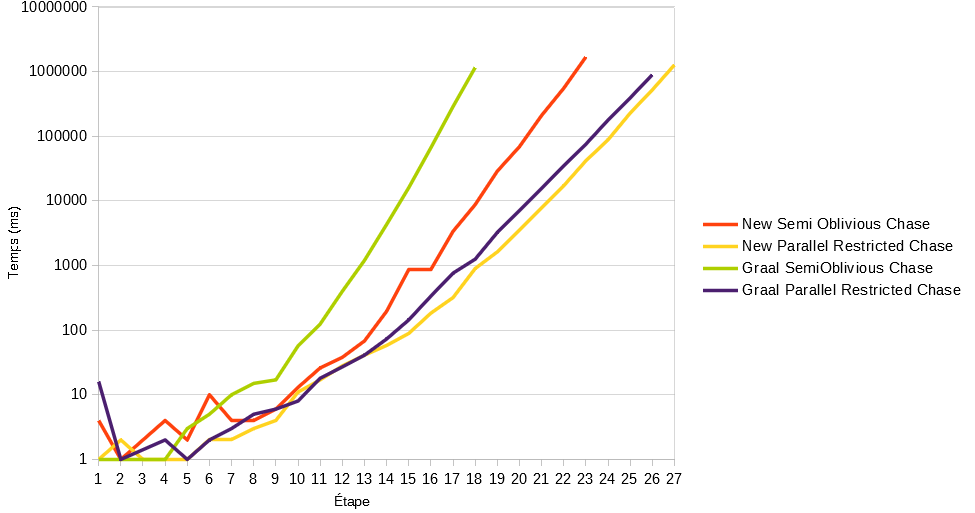
\includegraphics[width=0.8\textwidth]{img/exampleoldnew.png}
    }
    \only<2>{
        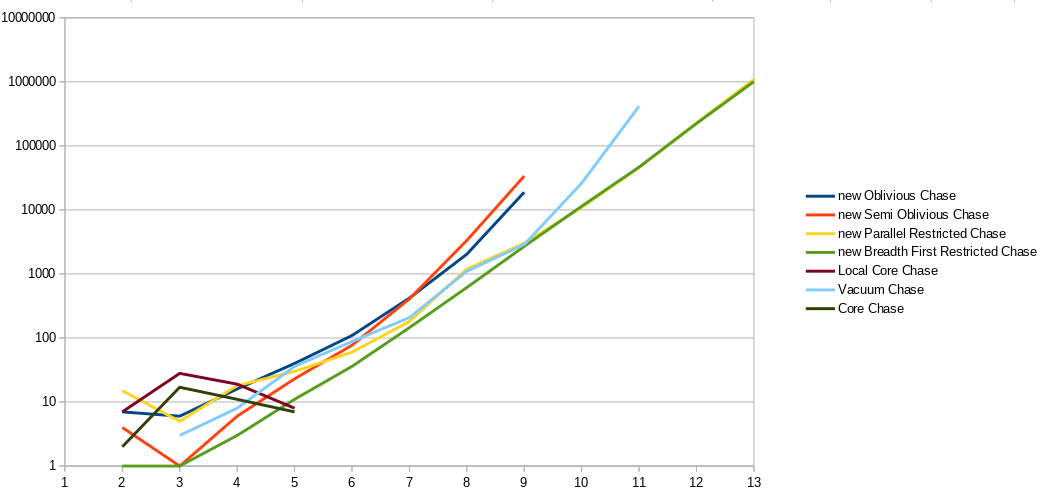
\includegraphics[width=0.9\textwidth]{img/ex0_exec_times.png}
    }
    \only<3>{
        %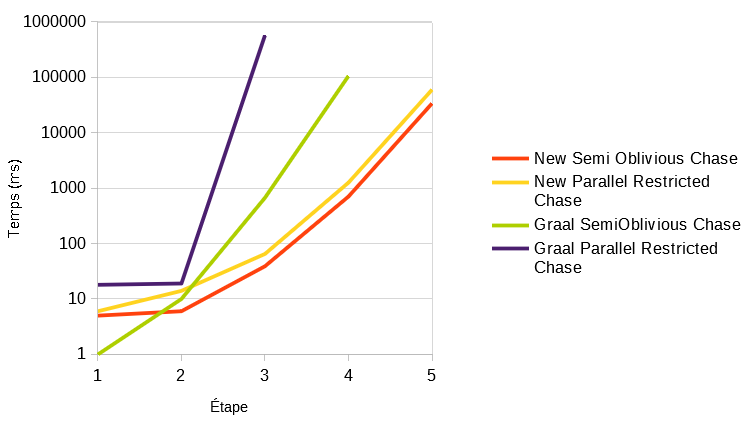
\includegraphics[width=0.7\textwidth]{img/ex11oldnew.png}
        \begin{table}[H]
\begin{center}
\begin{tabular}{|c|c|c|c|c|} 
    \hline
    $\mathcal{KB}$/Étape & \shortstack{New \\ Semi-oblivious}  & \shortstack{Graal \\ Semi-oblivious} & \shortstack{New \\ Restricted} & \shortstack{Graal \\ Restricted} \\
    \hline
     \hline
    $\mathcal{KB}_A$/6 & 55987 & 55987 & 1375 & 1375 \\ 
     \hline
    $\mathcal{KB}_B$/5 & 111111 & 111111 & 3851 & 3851 \\ 
    \hline
    $\mathcal{KB}_C$/4 & 107754 & 107754 & 21882 & 21882 \\ 
    \hline
    $\mathcal{KB}_D$/4 & \color{green}1556 & \color{green}1556 & \color{green}1556 & \color{red}152324 \\
    \hline
    $\mathcal{KB}_E$/13 & 754 & 754 & 332 & 332 \\ 
     \hline
    $\mathcal{KB}_F$/4 & 48315 & 48315 & 24918 & 24918 \\ 
     \hline 
\end{tabular}    
\caption {Comparaison des \textit{chases} par nombr \label{tab:faitsoldnew}
\end{center}
\end{table}
    }
    \end{center}
\end{frame}


\section{Règles}
    \frame{\frametitle{Table des matières}\tableofcontents[currentsection]}
    \begin{frame}{Redondance dans les règles}

    Deux formes de redondances statiques étudiées :

    \begin{itemize}
        \item Les redondances intra-règle 
        \item Les redondances inter-règle 
    \end{itemize}
    
   
\end{frame}

 
    \subsection{Redondances intra-règles}
    \begin{comment}



\begin{frame}{Redondances intra-règle}
     Deux formes de redondances statiques étudiées :

    \begin{itemize}
    \color{red}
        \item Les redondances intra-règle 
        \color{black}
        \item Les redondances inter-règle 
       
    \end{itemize}
\end{frame}{}

\end{comment}

\begin{frame}{Redondances intra-règle}

    Il existe 2 formes de redondances intra-règle :

    \begin{itemize}
        \item Les redondances dans le corps de la règle 
        \item Les redondances de la tête sur le corps et dans la tête de la règle
    \end{itemize}
    
   
\end{frame}

\begin{frame}{Redondances intra-règle}

    Il existe 2 formes de redondances intra-règle :

    \begin{itemize}
        \color{red}
        \item Les redondances dans le corps de la règle 
        \color{black}
        \item Les redondances de la tête sur le corps et dans la tête de la règle
    \end{itemize}
    
   \begin{block}{Exemple}
        Soit la règle $R = $ \color{blue}p(X)\color{black} $\land$ \color{red}$ p(Y) $\color{black} $\xrightarrow{} \exists Z.q($\color{blue}X\color{black}$,Z)$.
    \end{block}
    \begin{tikzpicture}[->,>=stealth,shorten >=1pt,auto,node distance=2.5cm,
               thick,main node/.style={circle,draw,font=\Large\bfseries,scale=0.6}]
    \node[main node] (1) [blue] {$X$};
  \node[main node] (2) [below of=1, red] {$Y$};
  \node[main node] (3) [right of=2] {$Z$};

  \path
    (1) edge [loop above, blue] node {p} (1)
    (1) edge node {q} (3)
    (2) edge [loop above, red] node {p} (2)
  ;
\end{tikzpicture}

On obtient $R' = p(X) \xrightarrow{} \exists Z.q(X,Z)$.
   
\end{frame}


\begin{frame}{Redondances intra-règle}

    Il existe 2 formes de redondances intra-règle :

    \begin{itemize}
       
        \item Les redondances dans le corps de la règle 
         \color{red}
     
        \item Les redondances de la tête sur le corps et dans la tête de la règle
           \color{black}
    \end{itemize}

    \begin{block}{Exemple}
        Soit la règle $R = $\color{blue}p(X,Y)\color{black} $\xrightarrow{} \exists Z,S,T. p($\color{blue}Y\color{black}$,Z) \land $ \color{red} $p(T,Z) \land p(S,T)$ \color{black}.
    \end{block}
    
 \begin{tikzpicture}[->,>=stealth,shorten >=1pt,auto,node distance=2.5cm,
                thick,main node/.style={circle,draw,font=\Large\bfseries,scale=0.6}]
  \node[main node] (1) [blue] {$X$};
  \node[main node] (2) [right of=1, blue] {$Y$};
  \node[main node] (3) [right of=2] {$Z$};
  \node[main node] (4) [right of=3, red] {$T$};
  \node[main node] (5) [right of=4, red] {$S$};

  \path
    (1) edge [blue] node {p} (2) 
    (2) edge node {p} (3)
    (4) edge [red] node {p} (3)
    (5) edge [red] node {p} (4)
  ;
\end{tikzpicture}

 \begin{tikzpicture}[->,>=stealth,shorten >=1pt,auto,node distance=2.5cm,
                thick,main node/.style={circle,draw,font=\Large\bfseries,scale=0.6}]
  \node[main node] (1) [blue] {$X$};
  \node[main node] (2) [right of=1, blue] {$Y$};
  \node[main node] (3) [right of=2] {$Z$};

  \path
    (1) edge [blue] node {p} (2)
    (2) edge node {p} (3)
  ;
\end{tikzpicture}

On obtient la règle $R' = p(X,Y) \xrightarrow{} \exists Z.p(Y,Z)$

\end{frame}


%
%\begin{frame}[fragile]{Redondances intra-règle}
%    Les redondances du corps dans le corps de la règle :
    
%    \begin{block}{Exemple}
%        Soit la règle $R = p(X) \land p(Y) \xrightarrow{} q(X,Z)$.
%    \end{block}
    
%    Si $R$ est appliquée on aura la base de faits $\mathcal{F} = \{p(X),  p(Y), q(X,Z_1)\}$.
    
 %     \begin{block}{Le graphe représentant $\{p(X),  p(Y), q(X,Z_1)\}$}
 %    \begin{tikzpicture}[->,>=stealth,shorten >=1pt,auto,node distance=2.5cm,
%                thick,main node/.style={circle,draw,font=\Large\bfseries,scale=0.6}]
%    \node[main node] (1) {$X$};
%  \node[main node] (2) [below of=1] {$Y$};
%  \node[main node] (3) [right of=2] {$Z_1$};

%  \path
%    (1) edge [loop above] node {p} (1)
%    (1) edge (3)
%    (2) edge [loop above] node {p} (2)
%  ;
%\end{tikzpicture}
%\end{block} 
%\end{frame}


%\begin{frame}{Redondances intra-règle}
    
%    Les redondances du corps dans le corps de la règle :
    
%    \begin{block}{Exemple}
%        Soit la règle $R = p(X) \land p(Y) \xrightarrow{} q(X,Z)$.
%    \end{block}
    
%    Si on calcul le \textit{core} à la base de faits $\mathcal{F}$ on obtient $\mathcal{F}'  = \{p(X), q(X,Z_1)\}$.
    
%     \begin{block}{Le graphe représentant $\{p(X),  q(X,Z_1)\}$}
%     \begin{tikzpicture}[->,>=stealth,shorten >=1pt,auto,node distance=2.5cm,
 %               thick,main node/.style={circle,draw,font=\Large\bfseries,scale=0.6}]
 %   \node[main node] (1) {$X$};
 % \node[main node] (3) [right of=2] {$Z_1$};

  %\path
  %  (1) edge [loop above] node {p} (1)
  %  (1) edge (3)
 % ;
%\end{tikzpicture}
%\end{block} 
    
%\end{frame}
    


\begin{frame}{Redondances intra-règle}
   
    \begin{block}{Comment supprimer ces redondances ? }
        On va utiliser le \textit{Core}. 
    \end{block}
    
        
 \begin{tikzpicture}[->,>=stealth,shorten >=1pt,auto,node distance=2.5cm,
                thick,main node/.style={circle,draw,font=\Large\bfseries,scale=0.6}]
  \node[main node] (1) [blue] {$X$};
  \node[main node] (2) [right of=1, blue] {$Y$};
  \node[main node] (3) [right of=2] {$Z$};
  \node[main node] (4) [right of=3, red] {$T$};
  \node[main node] (5) [right of=4, red] {$S$};

  \path
    (1) edge [blue] node {p} (2) 
    (2) edge node {p} (3)
    (4) edge [red] node {p} (3)
    (5) edge [red] node {p} (4)
  ;
\end{tikzpicture}
    
  
    
\end{frame}



%\begin{frame}{Redondances intra-règles}

  %  Algorithmes pour supprimer les redondances intra-règles :
    
%   \begin{itemize}
 %       \item On calcul le \textit{core} sur le corps de la règle en gelant la frontière
 %       \item On calcul le \textit{core} sur le nouveau corps gelé et la tête de la règle
 %       \item Si la tête est vide on supprime la règle de la base de règles
 %   \end{itemize}
   
%\end{frame}

%\begin{frame}{Redondances intra-règles}

 %   Algorithmes pour supprimer les redondances intra-règles :
    
 %   \begin{itemize}
 %       \item On calcul le \textit{core} sur le corps de la règle en gelant la frontière
 %       \item On calcul le \textit{core} sur le nouveau corps gelé et la tête de la règle
  %      \item Si la tête est vide on supprime la règle de la base de règles
  %  \end{itemize}
    
  %  \begin{block}{Exemple}
  %      Soit la règle $R =  p(X,Y) \land p(X,U) \xrightarrow{} p(Y,Z) \land p(T,Z) \land p(S,T)$
%    \end{block}
   
%\end{frame}

%\begin{frame}{Redondances intra-règles}

 %   Algorithmes pour supprimer les redondances intra-règles :
    
 %   \begin{itemize}
 %       \color{red}
 %       \item On calcul le \textit{core} sur le corps de la règle en gelant la frontière
 %       \color{black}
 %       \item On calcul le \textit{core} sur le nouveau corps gelé et la tête de la règle
 %       \item Si la tête est vide on supprime la règle de la base de règles
 %   \end{itemize}
    
 %   \begin{block}{Exemple}
%        Soit la règle $R =  p(X,Y) \land p(X,U) \xrightarrow{} p(Y,Z) \land p(T,Z) \land p(S,T)$
 %       On gèle la frontière de $R$, ici : $Y$.
 %       Puis on calcul le \textit{core} sur le corps : $\{p(X,Y), p(X,U)\}$ pour obtenir : $\{p(X,Y)\}$. 
 %%        \begin{tikzpicture}[->,>=stealth,shorten >=1pt,auto,node distance=2.5cm,
  %              thick,main node/.style={circle,draw,font=\Large\bfseries,scale=0.6}]
 % \node[main node] (1) {$X$};
 % \node[main node] (2) [right of=1] {$Y$};
%  \node[main node] (3) [left of=1] {$U$};

 %% \path
 %   (1) edge (2)
 % ;
 % \end{tikzpicture}
 
 %   Dont le \textit{core} est : 
 %   \begin{tikzpicture}[->,>=stealth,shorten >=1pt,auto,node distance=2.5cm,
%                thick,main node/.style={circle,draw,font=\Large\bfseries,scale=0.6}]
%  \node[main node] (1) {$X$};
%  \node[main node] (2) [right of=1] {$Y$};

 % \path
 %   (1) edge (2)
 % ;
%  \end{tikzpicture}
%    \end{block}
   
%\end{frame}

%\begin{frame}{Redondances intra-règles}

  %  Algorithmes pour supprimer les redondances intra-règles :
    
  %  \begin{itemize}
%        \item On calcul le \textit{core} sur le corps de la règle en gelant la frontière
 %       \color{red}
  %      \item On calcul le \textit{core} sur le nouveau corps gelé et la tête de la règle
  %      \color{black}
  %      \item Si la tête est vide on supprime la règle de la base de règles
 %   \end{itemize}
    
 %   \begin{block}{Exemple}
 %       Soit la règle $R' =  p(X,Y) \xrightarrow{} p(Y,Z) \land p(T,Z) \land p(S,T)$
 %       On gèle la frontière de $R'$, ici : $Y$.
 %       Puis on calcul le \textit{core} sur le corps et la tête : $\{p(X,Y)\} \bigcup \{p(Y,Z), p(T,Z), p(S,T)\}$. 
 %        \begin{tikzpicture}[->,>=stealth,shorten >=1pt,auto,node distance=2.5cm,
 %               thick,main node/.style={circle,draw,font=\Large\bfseries,scale=0.6}]
 %  \node[main node] (1) {$X$};
  %\node[main node] (2) [right of=1] {$Y$};
%  \node[main node] (3) [right of=2] {$Z$};
%  \node[main node] (4) [right of=3] {$T$};
%  \node[main node] (5) [right of=4] {$S$};

%  \path
%    (1) edge (2)
%    (2) edge (3)
%    (4) edge (3)
%    (5) edge (4)
%  ;
%  \end{tikzpicture}
 
 %   Dont le \textit{core} est : 
 %   \begin{tikzpicture}[->,>=stealth,shorten >=1pt,auto,node distance=2.5cm,
 %               thick,main node/.style={circle,draw,font=\Large\bfseries,scale=0.6}]
%  \node[main node] (1) {$X$};
%  \node[main node] (2) [right of=1] {$Y$};
%  \node[main node] (3) [right of=2] {$Z$};

%  \path
%    (1) edge (2)
%    (2) edge (3)
%  ;
%  \end{tikzpicture}
%    \end{block}
   
%\end{frame}

%\begin{frame}{Redondances intra-règles}

%    Algorithmes pour supprimer les redondances intra-règles :
    
 %   \begin{itemize}
%        \item On calcul le \textit{core} sur le corps de la règle en gelant la frontière
%        
%  \item On calcul le \textit{core} sur le nouveau corps gelé et la tête de la règle
%        \color{red}
%        \item Si la tête est vide on supprime la règle de la base de règles
%        \color{black}
%    \end{itemize}
    
    
 %   \begin{block}{Exemple}
 %       Soit la règle $R =  p(X,Y) \xrightarrow{} p(X,Z)$
 %       On gèle la frontière de $R$, ici : $X$.
 %       Puis on calcul le \textit{core} sur le corps et la tête : 
 %        \begin{tikzpicture}[->,>=stealth,shorten >=1pt,auto,node distance=2.5cm,
  %              thick,main node/.style={circle,draw,font=\Large\bfseries,scale=0.6}]
%   \node[main node] (1) {$X$};
%  \node[main node] (2) [right of=1] {$Y$};
%  \node[main node] (3) [below of=2] {$Z$};

 % \path
 %   (1) edge (2)
 %   (1) edge (3)
%  ;
 % \end{tikzpicture}
 
 %   Dont le \textit{core} est : 
%    \begin{tikzpicture}[->,>=stealth,shorten >=1pt,auto,node distance=2.5cm,
 %               thick,main node/.style={circle,draw,font=\Large\bfseries,scale=0.6}]
 % \node[main node] (1) {$X$};
 % \node[main node] (2) [right of=1] {$Y$};

%  \path
%    (1) edge (2)
%  ;
  
 
%  \end{tikzpicture}
%  On obtient $R' = p(X,Y) \xrightarrow{}$ sans redondances mais qui ne produit plus rien.
%    \end{block}
   
%\end{frame}
    \subsection{Redondances inter-règles}
    \begin{frame}{Redondances inter-règles}
    Si une règle $R$ est redondante à une base de règles $\mathcal{R}$ alors elle peut être inférée par $\mathcal{R} \backslash R$.
    
    \begin{block}{Exemple}
        Soit la base de règles $\mathcal{R} = \{ R_1 = p(X) \xrightarrow{} q(X), R_2 = p(X) \xrightarrow{} t(X), R_3 = q(x) \xrightarrow{} t(X)\}$
    \end{block}
    
    Nous verrons lors de l'application de l'algorithme sur cet exemple que $R_2$ peut être inférée par $\mathcal{R} \backslash R_2$.
    
\end{frame}

\begin{frame}{Redondances inter-règles}
   
   Algorithme pour supprimer les redondances inter-règles :
    
    \begin{itemize}
        \item On ajoute le corps de $R$ à une base de fait $\mathcal{F}$
        \item On construit la base de connaissance $\mathcal{KB} = \{\mathcal{F}, \mathcal{R} \backslash R \}$
        \item On sature $\mathcal{KB}$ et on obtient $\mathcal{F}^*$ la base de faits saturée
        \item On gèle la frontière de $R$ et on cherche si la tête de $R$ se trouve dans $\mathcal{F}^*$.
    \end{itemize}
    
    La saturation d'une base de faits étant infinie, il est préférable de prévoir un arrêt au bout d'un certains nombre d'étapes.
    
\end{frame}

\begin{comment}


\begin{frame}{Redondances inter-règles}
   
   Algorithme pour supprimer les redondances inter-règles :
    
    \begin{itemize}
        \color{red}
        \item On ajoute le corps de $R$ à une base de fait $\mathcal{F}$
        \item On construit la base de connaissance $\mathcal{KB} = \{\mathcal{F}, \mathcal{R} \backslash R \}$
        \color{black}
        \item On sature $\mathcal{KB}$ et on obtient $\mathcal{F}^*$ la base de faits saturée
        \item On gèle la frontière de $R$ et on cherche si la tête de $R$ se trouve dans $\mathcal{F}^*$
    \end{itemize}
    
    \begin{block}{Exemple}
          Soit la base de règles $\mathcal{R} = \{ R_1 = p(X) \xrightarrow{} q(X), R_2 = p(X) \xrightarrow{} t(X), R_3 = q(x) \xrightarrow{} t(X)\}$. On commence par traiter $R_1$ et on construit la base de connaissances $\mathcal{KB} = \{ \{p(X)\}, \mathcal{R} \backslash R_1\}$.
    \end{block}
    
\end{frame}

\begin{frame}{Redondances inter-règles}
   
   Algorithme pour supprimer les redondances inter-règles :
    
    \begin{itemize}
        \item On ajoute le corps de $R$ à une base de fait $\mathcal{F}$
        \item On construit la base de connaissance $\mathcal{KB} = \{\mathcal{F}, \mathcal{R} \backslash R \}$
        \color{red}
        \item On sature $\mathcal{KB}$ et on obtient $\mathcal{F}^*$ la base de faits saturée
        \item On gèle la frontière de $R$ et on cherche si la tête de $R$ se trouve dans $\mathcal{F}^*$.
        \color{black}
    \end{itemize}
    
    \begin{block}{Exemple}
          Soit la base de règles $\mathcal{R} \backslash R_1 = \{R_2 = p(X) \xrightarrow{} t(X), R_3 = q(x) \xrightarrow{} t(X)\}$. On sature $\mathcal{F} = \{p(X)\}$ et on obtient $\mathcal{F}^* = \{p(X), t(X)\}$. Ici $q(X)$ n'appartient pas à $\mathcal{F}^*$ donc $R_1$ n'est pas redondante.
    \end{block}
    
\end{frame}

\end{comment}


\begin{frame}{Redondances inter-règles}
   
   Algorithme pour supprimer les redondances inter-règles :
    
    \begin{itemize}
        \color{red}
        \item On ajoute le corps de $R$ à une base de fait $\mathcal{F}$
        \item On construit la base de connaissance $\mathcal{KB} = \{\mathcal{F}, \mathcal{R} \backslash R \}$
        \color{black}
        \item On sature $\mathcal{KB}$ et on obtient $\mathcal{F}^*$ la base de faits saturée
        \item On gèle la frontière de $R$ et on cherche si la tête de $R$ se trouve dans $\mathcal{F}^*$.
    \end{itemize}
    
    \begin{block}{Exemple}
          Soit la base de règles $\mathcal{R} = \{ R_1 = p(X) \xrightarrow{} q(X), R_2 = p(X) \xrightarrow{} t(X), R_3 = q(x) \xrightarrow{} t(X)\}$. On traite $R_2$ et on construit la base de connaissances $\mathcal{KB} = \{ \{p(X)\}, \mathcal{R} \backslash R_2\}$.
    \end{block}
    
\end{frame}

\begin{frame}{Redondances inter-règles}
   
  Algorithme pour supprimer les redondances inter-règles :
    
    \begin{itemize}
        \item On ajoute le corps de $R$ à une base de fait $\mathcal{F}$
        \item On construit la base de connaissance $\mathcal{KB} = \{\mathcal{F}, \mathcal{R} \backslash R \}$
        \color{red}
        \item On sature $\mathcal{KB}$ et on obtient $\mathcal{F}^*$ la base de faits saturée
        \item On gèle la frontière de $R$ et on cherche si la tête de $R$ se trouve dans $\mathcal{F}^*$.
        \color{black}
    \end{itemize}
    
    \begin{block}{Exemple}
          Soit la base de règles $\mathcal{R} \backslash R_2 = \{ R_1 = p(X) \xrightarrow{} q(X), R_3 = q(x) \xrightarrow{} t(X)\}$. On sature $\mathcal{F} = \{p(X)\}$ et on obtient $\mathcal{F}^* = \{p(X), q(X), t(X)\}$. Ici $t(X)$ appartient à $\mathcal{F}^*$ donc $R_2$ est redondante. On peut donc la supprimer de la base de règles.
    \end{block}
    
\end{frame}


\begin{frame}{Redondances inter-règles}
   
  Algorithme pour supprimer les redondances inter-règles :
    
    \begin{itemize}
        \item On ajoute le corps de $R$ à une base de fait $\mathcal{F}$
        \item On construit la base de connaissance $\mathcal{KB} = \{\mathcal{F}, \mathcal{R} \backslash R \}$
     
        \item On sature $\mathcal{KB}$ et on obtient $\mathcal{F}^*$ la base de faits saturée
        \item On gèle la frontière de $R$ et on cherche si la tête de $R$ se trouve dans $\mathcal{F}^*$.
   
    \end{itemize}
    
    \begin{block}{Exemple}
    $R_1$ et $R_3$ n'est pas redondante. 
        Soit la nouvelle base de règles $\mathcal{R}' = \{ R_1 = p(X) \xrightarrow{} q(X), R_3 = q(x) \xrightarrow{} t(X)\}$ sans redondance inter-règles.
    \end{block}
    
\end{frame}


\begin{comment}
\begin{frame}{Redondances inter-règles}
   
   Algorithme pour supprimer les redondances inter-règles :
    
    \begin{itemize}
        \color{red}
        \item On ajoute le corps de $R$ à une base de fait $\mathcal{F}$
        \item On construit la base de connaissance $\mathcal{KB} = \{\mathcal{F}, \mathcal{R} \backslash R \}$
        \color{black}
        \item On sature $\mathcal{KB}$ et on obtient $\mathcal{F}^*$ la base de faits saturée
        \item On gèle la frontière de $R$ et on cherche si la tête de $R$ se trouve dans $\mathcal{F}^*$.
    \end{itemize}
    
    \begin{block}{Exemple}
          Soit la base de règles $\mathcal{R}' = \{ R_1 = p(X) \xrightarrow{} q(X), R_3 = q(x) \xrightarrow{} t(X)\}$. On traite $R_3$ et on construit la base de connaissances $\mathcal{KB} = \{ \{q(X)\}, \mathcal{R} \backslash R_3\}$.
    \end{block}
    
\end{frame}

\begin{frame}{Redondances inter-règles}
   
   Algorithme pour supprimer les redondances inter-règles :
    
    \begin{itemize}
        \item On ajoute le corps de $R$ à une base de fait $\mathcal{F}$
        \item On construit la base de connaissance $\mathcal{KB} = \{\mathcal{F}, \mathcal{R} \backslash R \}$
        \color{red}
        \item On sature $\mathcal{KB}$ et on obtient $\mathcal{F}^*$ la base de faits saturée
        \item On gèle la frontière de $R$ et on cherche si la tête de $R$ se trouve dans $\mathcal{F}^*$.
        \color{black}
    \end{itemize}
    
    \begin{block}{Exemple}
          Soit la base de règles $\mathcal{R}' \backslash R_3 = \{ R_1 = p(X) \xrightarrow{} q(X)$. On sature $\mathcal{F} = \{q(X)\}$ et on obtient $\mathcal{F}^* = \mathcal{F}$. Ici $t(X)$ n'appartient pas à $\mathcal{F}^*$ donc $R_3$ n'est pas redondante. 
    \end{block}
    
\end{frame}




\begin{frame}{Redondances inter-règles}
   
   Algorithme pour supprimer les redondances inter-règles :
    
    \begin{itemize}
        \color{red}
        \item On ajoute le corps de $R$ à une base de fait $\mathcal{F}$
        \item On construit la base de connaissance $\mathcal{KB} = \{\mathcal{F}, \mathcal{R} \backslash R \}$
        \color{black}
        \item On sature $\mathcal{KB}$ et on obtient $\mathcal{F}^*$ la base de faits saturée
        \item On gèle la frontière de $R$ et on cherche si la tête de $R$ se trouve dans $\mathcal{F}^*$
    \end{itemize}
    
    \begin{block}{Exemple}
         La base de règles $\mathcal{R} = \{ R_1 = p(X) \xrightarrow{} q(X), R_2 = p(X) \xrightarrow{} t(X), R_3 = q(x) \xrightarrow{} t(X)\}$ devient $\mathcal{R}' = \{ R_1 = p(X) \xrightarrow{} q(X), R_3 = q(x) \xrightarrow{} t(X)\}$ sans redondances inter-règles.
    \end{block}
    
\end{frame}

\end{comment}
    %\subsection{Expérimentations}
    %\begin{frame}{Expérimentations sur des bases de règles}
    Un algorithme général se découperait en deux phases :
    \begin{itemize}
        \item Phase 1 : traitement des redondances intra-règles
        \item Phase 2 : traitement des redondances inter-règles.
    \end{itemize}
    
   
\end{frame}
    \subsection{Démonstration}
        %\frame{\frametitle{Table des matières}\tableofcontents[currentsection]}
        \begin{frame}{Démonstration}
    Démonstration d'une suppression de redondances dans une base de règles.
\end{frame}
\section{Conclusion}
    \begin{frame}{Conclusion}
\begin{block}{Réalisation de nos objectifs :}
    \begin{itemize}
        \item Étude d'algorithmes de chaînage avant ;
        \item analyse des chaînages avant dans la librairie Graal ;
        \item nouvelle structure mieux à même de répondre aux évolutions futures de la bibliothèque ;
        \item implementations et premières expérimentations ;
        \item étude des redondances dans les bases de règles et création d'algorithmes supprimant ces redondances.
    \end{itemize}
\end{block}
    
    % \begin{itemize}
    %     \item tester sur des KB plus grande
    %     \item tester d'autres algos
    %     \item tester le vacuum chase
        
    % \end{itemize}
\end{frame}

\begin{frame}{Conclusion}
    \begin{block}{Ce que le projet nous a apporté}
        \begin{itemize}
            \item initiation à la recherche ;
            \item ingénierie logicielle, UML et Java.
        \end{itemize} 
    \end{block}
    \begin{block}{Perspectives}
        \begin{itemize}
            \item Expérimentation à grande échelle à l'aide des bases de connaissances créées par la communauté scientifique;
            \item mettre au point différent algorithme de \textit{chases}.
        \end{itemize}
    \end{block}
\end{frame}

\end{document}